\chapter{Item Response Theory Background} \label{ch:irt_background}

In educational measurement, a common goal is to quantify the knowledge of students from the results of some assessment. In a classroom setting, grades are typically assigned based on the percentage of questions answered correctly by a student assignments. The letter grades assigned from these percentages can serve as a naive measure of student knowledge; ``A'' students have completely mastered the material, ``B'' students have a good grasp of material, ``C'' students are fairly average, and ``D'' and ``F'' students have significant gaps in their knowledge.

The practice of evaluating student ability purely from a raw percentage score is known as true score theory \cite{thissen}. But there are clear issues with this approach. Not all questions on an exam or homework assignment is created equally: some questions are easier, and some more difficult. Consider a scenario where two students both answer 17 out of 20 questions correctly on a test for a raw score of $85\%$. But if Student A answered questions 1, 8, and 9 wrong while Student B answered 4, 17, and 20 incorrectly, it is not likely that that Student A and Student B possess the same level of knowledge. For example, questions 1, 8, and 9 could be much more difficult than questions 4, 17, and 20. Additionally, the two sets of problems could cover different types of material. True score theory does not account for either of these situations, and naively quantifies the knowledge of Student A and Student B as equal.

More sophisticated methods have been studied which attempt to more accurately quantify student learning. Cognitive Diagnostic Models (CDM) (TODO: citation) aim to classify whether students possess mastery of a given skill or not. This discrete classification can be useful in determining whether or not a student meets a prerequisite, or deciding whether or not they are ready to move on to the next level of coursework. We focus instead on Item Response Theory, where student knowledge is assumed to be continuous.

\section{Item Response Theory}
Item Response Theory (IRT) is a field of quantitative psychology which uses statistical models to model student ability \cite{lord1968}. These models often give the probability of a question being answered correctly as a function of the student's ability. In IRT, it is assumed that each student, indexed by $j$, possesses some continuous latent ability $\theta_j$. The term ``latent ability'' is synonymous with ``knowledge''or ``skill.'' Often, it is assumed that amongst the population of students, $\theta_j \sim \mathcal{N}(0,1)$ \cite{thissen}. 

In this work, we often consider the case where each student has multiple latent abilities. For example, in the context of an elementary math exam, we may wish to measure the four distinct skills ``add'', ``subtract'', ``multiply'', and ``divide.'' This scenario is referred to as multidimensional item response theory, and we write the set of student $j$'s $K$ latent abilities as a vector $\Theta_j = (\theta_{1j}, \theta_{2j}, \ldots, \theta_{Kj})^\top$. It is then assumed that the latent abilities of students follow some multivariate Gaussian distirbution, $\mathcal{N}(0, \Sigma)$. For simplicity, the covariance matrix $\Sigma$ is often taken to be the identity matrix, making each latent skill independent of one another.

Note that $\Theta_j$ is not directly observable in any way. Instead, a common goal is to infer student's knowledge $\Theta_j$ from on their responses on some assessment containing $n$ questions, referred to as items. A student's set of responses can be written as a binary $n$-dimensional vector $\vec u_j = (u_{1j}, u_{2j}, \ldots, u_{nj})^\top$, where 
\begin{equation}
  u_{ij} = \begin{cases} 1 & \text{if student } j \text{ answers item } i \text{ correctly} \\0 & \text{otherwise} \end{cases} 
  \label{eq:responses}
\end{equation}
IRT models aim to model the probability of a student answering a particular question correctly, so that the probability of student $j$ answering item $i$ correctly is given by some function of $\Theta_j$:
\begin{equation}
  P(u_{ij} = 1 | \Theta_j) = f(\Theta_j; V_i)
\end{equation}
where $V_i$ is a set of parameters associated with item $i$. In general, $f:\R^K \to [0,1]$ is some continuous function which is strictly increasing with respect to $\Theta_j$.

\begin{figure}[h]
  \centering
  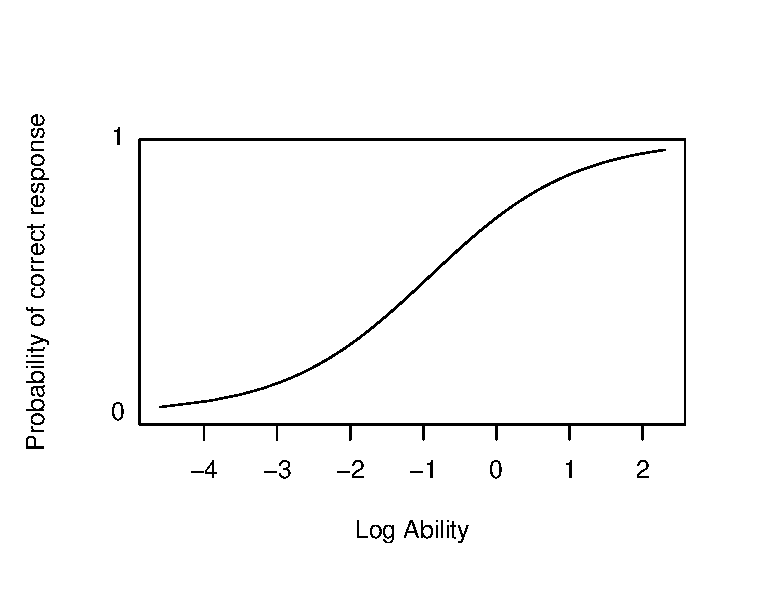
\includegraphics[width=.6\textwidth, angle=90]{img/logistic_1param_icc.eps}
  \caption{An item characteristic curve visualizes the relation between a student's ability and the probability of answering an item correctly.}
  \label{fig:icc}
\end{figure}

In the following sections, we describe various candidates for the function $f$. Though each is presented in the context of single-dimensional IRT ($K = 1$), they can all be easily adapted to higher dimensions.

\subsection{Rasch Model}
One of the first models was proposed by Georg Rasch in 1960. Rasch asserted that the probability of a student answering an item correctly is a function of the ratio $\xi / \d$, where $\xi > 0$ represents the student's knowledge, and $\d > 0$ quantifies the difficulty of an item. Consider the $\frac{\xi}{\xi + \d} = \frac{1}{1 + \d / \xi}$ and note that $\frac{\xi}{\xi + \d} \to 1$ as $\xi \to \infty$. After the reparametarization $\xi = e^{\theta}$ and $\d = e^{b}$, we arrive at the 1-Parameter Logistic Model, often referred to as the Rasch Model.
\begin{equation}
  P(u_{ij} = 1 | \theta_j; b_i) = \frac{1}{1 + e^{b_i - \theta_j}}
  \label{eq:rasch}
\end{equation}

Note that $\theta \in \R$ and $b \in \R$ still represent student ability and item difficulty, respectively. We can interpret the difficulty parameter $b$ as a threshold: when $\theta = b$, then the student has a $50\%$ chance of answering the question correctly. A plot of Equation \ref{eq:rasch} for a fixed item (fixed $b_i$) is shown in Figure \ref{fig:icc}. The horizontal axis represents $\log \theta$, and the vertical axis represents $P(u_{ij} = 1 | \theta, b_i)$. This type of graph is often referred to as an item characteristic curve (ICC).

\subsection{Normal Ogive Model}
\sideremark{*This section isn't very important to rest of work}
A slightly more sophisticated method for measuring student performance is the normal ogive model. We introduce a discrimination parameter, $a_i$, which quantifies the capability of item $i$ in distinguishing between students who have / have not mastered the knowledge concept $\theta$ \cite{thissen}. In other words, $a_i$ tells \textit{how much} of skill $\theta$ is required to answer item $i$ correctly. 

The normal ogive model give the probability of student $j$ answering item $i$ correctly as
\begin{equation}
  P(u_{ij} = 1 | \theta_j; a_i, b_i) = \frac{1}{\sqrt{2\pi}} \int_{-a_i \theta_j + b_i}^\infty e^{\frac{-z^{2}}{2}}dz
  \label{eq:ogive}
\end{equation}
Note the similarity between Equation \ref{eq:ogive} and the cumulative distribution function for a Gaussian distribution. The normal ogive model is popular among statisticians for this reason, but can be difficult to use for parameter estimation. 

\subsection{2-Parameter Logistic Model}
The model which this work focuses on most is the 2-parameter logistic (2PL) model. Like the normal ogive model, the 2PL model uses both the discrimination and difficulty item parameters. The probability of student $j$ answering item $i$ correctly is given by
\begin{equation}
  P(u_{ij} = 1 | \theta_j; a_i, b_i) = \frac{1}{1 + e^{-a_i \theta_j + b_i}}
  \label{eq:2PL}
\end{equation}
Equation \ref{eq:2PL} has the same form as that of the Rasch model in Equation \ref{eq:rasch}, but adds in the discrimination parameter $a_i$. If this parameter is scaled by 1.7, then the ICC from the normal ogive model differs from that of the 2PL model by $0.01$ \cite{baker_kim2004}. In a sense, we can consider the 2PL model to be a very good approximation of the normal ogive model. Due to the simple form of Equation \ref{eq:2PL}, using this model makes parameter estimation much easier.

\subsection{Multidimensional Item Response Theory}
The previously described statistical models can all be extended so that each student possesses $K$ latent traits. In multidimensional item response theory (MIRT), models give the probability of a correct answer as a function of the student ability vector $\Theta = (\theta_1,\ldots, \theta_K)^\top$. The generalization of \ref{eq:2PL} is given by the multidimensional logistic 2-parameter (ML2P) model:
\begin{equation}
P(u_{ij} = 1 | \Theta_j; \vec{a_i}, b_i) = \frac{1}{1 + \exp\left(-\vec{a_i}^\top \Theta_j + b_i\right)} = \frac{1}{\exp\left(-\sum_{k=1}^K a_{ik} \theta_{kj} + b_i \right)}
  \label{eq:ml2p}
\end{equation}
Here, the discrimination parameters $\vec{a_i} \in \R^K$ are given as vector, where each entry $a_{ik} \in \vec{a_i}$ quantifies \textit{how much} of skill $k$ is required to answer item $i$ correctly. The ML2P model is the main focus of this thesis.

TODO: mention MDISC and how this scales

In MIRT, it is convenient to notate the relationship between skills and items with binary matrix. Define the $Q$-matrix \cite{daSilva2018} $Q \in \{0,1\}^{n\times K}$ so that 
\begin{equation}
  q_{ik} = \begin{cases}
    1 & \text{if item } i \text{ requires skill } k\\
    0 & \text{otherwise}
  \end{cases}.
  \label{eq:q_matrix}
\end{equation}
In real applications, the $Q$-matrix is annotated by an expert in the field, as it is usually possible to discern the concepts need to answer an item correctly. In relation to the ML2P model (Equation \ref{eq:ml2p}), notice that if $q_{ik} = 0$, then $a_{ik} = 0$ as well. Though experts can produce a $Q$-matrix for a given assessment, the matrix of discrimination parameters $(a_{ik})_{i,k}$ can not be discovered so easily.

\section{IRT Parameter Estimation}
\sideremark{*How in-depth do these descriptions need to be? Could just give overall idea and describe weaknesses}

\subsection{Maximum Likelihood Estimation}
TODO: item parameter estimation

TODO: ability parameter estimation

\subsection{Joint Maximum Likelihood Estimation}


\subsection{Marginal Maximum Likelihood Estimation}
TODO: MMLE

TODO: EM 

\section{Artificial Neural Networks}
In recent years, artifical neural networks (ANN) have become an increasingly popular tool for machine learning problems. Though they have been around since the 1960's (TODO: citation), GPU technology has become more accessible and modern computers are more powerful, allowing anyone interested to train a basic neural network on their machine. ANN can be applied to a diverse set of problems, including regression, classification, computer vision, natural language processing, function approximation, data generation, and more (TODO: citations).

One of the biggest critiques of ANN is their black-box nature, meaning that the decision process that a trained model uses is typically not explainable by humans. As opposed to simpler methods such as decision trees or linear regression, neural networks are not interpretable. This makes them less desirable in certain applications where researchers wish to know \textit{why} a model predicts a particular data sample the way that it does. For example, if a financial institution is using data science methods to determine whether or not to approve someone's loan, the institution should be able to explain to the customer why they were denied. Most customers will not be satisfied with ``the computer told us so,'' and there is a possibility that a black-box neural network could learn and use features such as race or gender in its prediction, which is illegal in the United States (TODO: definitely need citation or delete).

The push for explainable AI have led researchers down two paths. One group has tried to incorporate deep learning methods with existing interpretable methods, in hopes of increasing the performance of explainable methods without sacrificing its interpretability (TODO: citation). Another option is to use a sort of hybrid learning, where interpretable models defer to a black-box model if they are not confident in their prediction \cite{rafique2020}. Others have started with deep models and cut back on complexity, making specific modifications which increase interpretability. For example, the loss function of a convolutional neural network can be adapted so that humans can understand the features extracted in the hidden layers \cite{zhang2018interpretable}. 

The field of education is an application which often desires interpretable models. Researchers often need to be able to point out specific details of decisions made by AI. A student deserves an answer to \textit{why} they failed a test, and a teacher should be given instructions on \textit{how} to fix the student's misconceptions.

\subsection{Autoencoders}
An autoencoder (AE) is a neural network where the input and output layers are the same shape. The objective for a given data point is to minimize the difference between the output, called the reconstruction, and the input. Typically, the middle hidden layers of an AE are of smaller dimension than the input space. In this way, autoencoders are an unsupervised learning technique for (nonlinear) dimension reduction. Mathematically, we can define an autoencoder in two parts as follows.

For an input $x \in \R^n$, define the \textit{encoder} as a function $f: \R^n \to \R^m$ mapping $x \mapsto z := f(x)$. Usually, $m < n$, and $z$ lies in a hidden feature space. The encoder sends an observed data point to its representation in a learned feature space. Define the \textit{decoder} as a function $g: \R^m \to \R^n$ mapping $z \mapsto \hat x := g(z)$. The decoder maps a hidden representation $z$ to a reconstruction of the encoder input. Note that in our case, the functions $f$ and $g$ are both parameterized by neural networks, each of which can have any number of hidden layers. The end-to-end autoencoder is then the function composition $\mathcal{A}(x):= g(f(x)): \R^n \to \R^n$. To train an AE, the loss function minimizes the difference between the input and output. This can be done in a number of ways, including the simple mean squared error loss
\begin{equation}
  \mathcal{L}(x) = || x - g(f(x))||_2^2
  \label{eq:mse}
\end{equation}
or cross-entropy loss for binary data
\begin{equation}
  \mathcal{L}(x) = \sum_{i=1}^n - x_i \log(g(f(x_i))) - (1-x_i)\log(1- g(f(x_i))).
  \label{eq:cross_entropy}
\end{equation}

Autoencoders with only a single hidden layer can be compared with nonlinear principal components analysis (PCA), and using linear activation functions allows for recovery of PCA loading vectors \cite{plaut2018}. AEs have clear applications in image compression straight out-of-the-box, and can be modified for more complicated problems. Denoising autoencoders \cite{vincent2008} are capable of processing noisy images and cleaning them up. To do this, they corrupt input data by deleting pixels at random and reconstructing the original image. Autoencoders can also be modified for data generation applications using a variational autoencoder.

\subsection{Variational Autoencoders}
\sideremark{*relevant sources: \cite{doersch2016} \cite{kingma2014} \cite{Blei2017}, infoVAE, ELBO, ``towards deeper understanding of VAE''}

% could talk about how Zhao et al (InfoVAE) show that if decoder is Gaussian, then maximizing ELBO makes the latent distribution bad - but I've shown this isn't the case in our model, where the decoder is Bernoulli.

The motivation for designing a variational autoencoder (VAE), introduced by Kingma and Welling \cite{kingma2014}, is different from regular autoencoders in that it is not rooted in neural networks. Rather, a probabilistic point of view provides the main source of motivation, and neural networks are a very common tool used to implement a VAE.

Consider a dataset $X = \{\vect x_i\}_{i=1}^N$, where each data point $\vect x_i \in \R^n$ is generated by a random process involving an unobserved variable $\vect z \in \R^d$. This unobserved variable is often referred to as ``latent code.'' It is assumed that to generate the observed data point $\vect x_i$, a value $\vect z_i$ is first sampled from a prior distribution $p_*(\vect z)$, and then $x_i$ is generated from a distribution $p_*(\vect x | \vect z)$.

From observing the dataset $X$, the latent variables $\vect z_i$ and parameters of the distributions $p_*(\vect z)$ and $p_*(\vect x | \vect z)$ are unknown. The goal of a VAE is to approximate these values, which leads to the ability to represent/encode data and generate new data. This should be done with a general algorithm that is unaffected by (i) intractability of the marginal likelihood $p(\vect x) = \int p(\vect z) \(\vect x | \vect z) d\vect z$ and (ii) large amounts of data. \sideremark{maybe point out this is a common problem with IRT param est methods} Note that (i) is important because if $p(\vect x)$ is intractable, and thus $p(\vect z | \vect x)$ is intractable, then the EM algorithm cannot be used.

In order to implement this task, two neural networks $q_\alpha(\vect z | \vect x)$ and $p_\beta(\vect x | \vect z)$ (probabilistic encoder and decoder, respectively) are used to approximate the unobservable true posterior distributions $p_{\alpha^*}(\vect z| \vect x)$ and $p_{\beta^*}(\vect x | \vect z)$. In the encoder/decoder, the indices $\alpha$ and $\beta$ reference settings of the trainable parameters of the neural network. Note that unlike a regular autoencoder, the probabilistic encoder $q_\alpha(\vect z | \vect x)$ of a VAE outputs a probability distribution for $\vect z$ given $\vect x$, rather than a single value.

\subsubsection{A note on Information Theory}
Before continuing, we introduce some ideas from information theory: entropy, cross-entropy, and KL-Divergence \cite{pattern_rec_book}. Consider a random variable $x$. For a particular value $x_0$, we can compute the amount of information gained from observing $x_0$ as $h(x_0) = -\log_2 p(x=x_0)$. When we use $\log_2$, the unit for information is ``bits,'' but any logarithm can be used. Note that we gain more information from observing a low-probability event than from observing a high-probability event. 

\textit{Entropy} is defined as the expectation of $h(x)$: the average amount of information that will be learned by observing a random $x$. So the entropy of the random variable $x$ is given as 
\begin{equation}
  H[p] = - \int p(x) \log p(x)dx
  \label{eq:entropy}
\end{equation}

Now assume that we also have access to a distribution $q(x)$ which approximates a possibly unknown $p(x)$. \textit{Cross-entropy} is the average amount of information needed to identify an event $x$ which was drawn from $q$ instead of $p$. Cross-entropy is given as
\begin{equation}
  H[p,q] = - \int p(x) \log q(x) dx
  \label{eq:xentropy}
\end{equation}

We can simply define \textit{Kullback-Leibler Divergence} (KL-Divergence) \cite{kullback1951} as 
\begin{equation}
  \mathcal{D}_{KL}\left[ p || q \right] = H[p] - H[p,q] = - \int p(x) \log \left(\frac{q(x)}{p(x)} \right)dx
  \label{eq:kl_div}
\end{equation}
Intuitively, KL-Divergence is amount of information which is lost if the approximating distribution $q(x)$ is used instead of the true distribution $p(x)$. However, KL-Divergence cannot be interpreted as a metric or as a distance between $p$ and $q$ because it is not symmetric -- in general, $\mathcal{D}_{KL}[p||q] \not = \mathcal{D}_{KL}[q||p]$. KL-Divergence is non-negative, and $\mathcal{D}_{KL}[p||q] = 0$ iff $p(x) = q(x)$.

\subsubsection{VAE Derivation}

We derive the desired loss function for a VAE. The log marginal likelihood is given as
\begin{equation}
  \log p_{\beta}(\vect x_1,\ldots,\vect x_N) = \sum_{i=1}^N \log p_{\beta}(\vect x_i)
  \label{eq:vae_marginal}
\end{equation}
Denoting $\vect x = \vect x_i$, we can rewrite each $p_{\beta}(\vect x_i)$ as \sideremark{I don't know the best way to index $p_\beta$ }
\begin{equation}
  \begin{split}
    \log p_{\beta}(\vect x) &= \int q_\alpha(\vect z |\vect x) \log p_{\beta} (\vect x)dz \\
    &= \int q_\alpha(\vect z | \vect x) \log \left( \frac{p_{\beta}(\vect z | \vect x) p_{\beta}(\vect x)}{p_{\beta}(\vect z | \vect x)} dz \right) \\
    &= \int q_\alpha(\vect z | \vect x) \log \left( \frac{p_{\beta}(\vect x, \vect z)}{p_{\beta}(\vect z | \vect x)} \right) dz\\
    &= \int q_\alpha(\vect z | \vect x) \left( \log \frac{q_\alpha(\vect z | \vect x)}{p_{\beta}(\vect z | \vect x)} + \log \frac{p_{\beta}(\vect x, \vect z)}{q_\alpha(\vect z | \vect x)}\right) dz \\
    &= \mathcal{D}_{KL}\left[ q_\alpha(\vect z |\vect x) || p_{\beta}(\vect z | \vect x) \right] + \int q_\alpha(\vect z | \vect x) \log \left( \frac{p_{\beta}(\vect x, \vect z)}{q_\alpha(\vect z | \vect x)} \right)dz \\
    &= \mathcal{D}_{KL}\left[ q_\alpha(\vect z |\vect x) || p_{\beta}(\vect z | \vect x) \right] + \mathbb{E}_{q_\alpha(\vect z | \vect x)}\left[ -\log q_\alpha(\vect z | \vect x) + \log p_{\beta}(\vect x, \vect z) \right] \\
    &= \mathcal{D}_{KL}\left[ q_\alpha(\vect z |\vect x) || p_{\beta}(\vect z | \vect x) \right] + \tilde{\mathcal{L}}(\alpha, \beta; \vect x)
\label{eq:vae_derive}
  \end{split}
\end{equation}

Note that in the final line, the first term is the KL-Divergence between the approximate and true posterior. Since we don't know the true posterior, we can't calculate this term. But notice that since KL-Divergence is always positive, and we can write 
\begin{equation}
  \begin{split}
    \log p_\beta (\vect x) \geq \tilde{\mathcal{L}}(\alpha, \beta; \vect x) = -\mathcal{D}_{KL}\left[ q_\alpha(\vect z | \vect x) || p_{\beta}(\vect z) \right] + \mathbb{E}_{q_\alpha(\vect z | \vect x)}\left[ \log p_{\beta}(\vect x | \vect z) \right]
  \label{eq:elbo}
\end{split}
\end{equation}

The term $\tilde{\mathcal{L}}(\alpha, \beta; \vect x)$ is referred to as the variational lower bound or Evidence Lower Bound (ELBO). Increasing the ELBO by varying the parameters $\alpha$ and $\beta$ will increase the marginal likelihood $\log p_\beta(\vect x)$, even though we ignore the term $\mathcal{D}_{KL}\left[ q_\alpha (\vect z | \vect x) || p_\beta(\vect z | \vect x) \right]$.

We take the ELBO $\tilde{\mathcal{L}}(\alpha,\beta; \vect x)$ to be a potential VAE objective function which we want to maximize. In Equation \ref{eq:elbo}, the first term gives the negative KL-Divergence between the probabilistic encoder $q_\alpha(\vect z | \vect x)$ and the true prior distribution of the latent code $p_\beta(\vect z)$. Note that unlike the true posterior $p_\beta(\vect z | \vect x)$, the true prior is known and is nearly always assumed to be independent Gaussian. 

For now, we assume that $\vect z \sim \mathcal{N}(0,I)$. Additionally, we assume that the encoder outputs a standard normal distribution. In Section \ref{sec:cov}, we propose architecture which fits the assumption that $\vect z \sim \mathcal{N}(\mu, \Sigma)$ and allows for the encoder to output a multivariate Gaussian distribution.

These assumptions make computing $\tilde{\mathcal{L}}(\alpha,\beta;\vect x)$ much easier. It can be shown \cite{doersch2016} that \sideremark{Should I show this?} the KL-Divergence between an independent Gaussian distribution and a standard normal distribution of dimension $K$ is calculated as
\begin{equation}
  \mathcal{D}_{KL}\left[ \mathcal{N}(\vect \mu_0, \vect \sigma_0^2I) || \mathcal{N}(0,I) \right] = \frac{1}{2}\sum_{k=1}^K \left( \mu_k^2 + \sigma_{0,k}^2 - 1 - \log(\sigma_{0,k}^2)\right)
  \label{eq:ind_gauss_kl}
\end{equation}
Note that the vectors $\vect \mu_0$ and $\vect \sigma_0^2$ are outputted by the encoder $q_\alpha(\vect z | \vect x_0)$, given the observed input $\vect x_0$. Since Equation \ref{eq:ind_gauss_kl} is in closed form, there is no difficulty in calculating the (possibly high-dimensional) integral that is usually required to compute KL-Divergence.

The second term in Equation \ref{eq:elbo} is similar to Equation \ref{eq:xentropy}, and depends on the probabilistic decoder $p_\beta(\vect x | \vect z)$, which is usually assumed to be either Gaussian or Bernoulli. Considering the desired application of educational measurement where data is given as binary responses, we assume that the decoder is Bernoulli. To deal with the expectation over $q_\alpha$, we simply sample $L$ times from $q_\alpha(\vect z | \vect x)$. In practice, it is often simplest to just choose $L=1$ \cite{kingma2014}. So then 
\begin{equation}
  \begin{split}
    \mathbb{E}_{q_\alpha(\vect z | \vect x)} \left[ \log p_\beta(\vect x | \vect z) \right] &\approx \frac{1}{L}\sum_{l=1}^L \log p_\beta(\vect x | \vect z^{(l)}) \\
    &\approx \log p_\beta(\vect x| \vect z^*) \\
    &= \log\left( \prod_{i=1}^n p_\beta(x_i = 1 | \vect z^*)^{x_i} \cdot p_\beta(x_i=0 | \vect z^*)^{x_i} \right) \\
  &= \sum_{i=1}^n x_i\log \hat x_i + (1-x_i)\log (1-\hat x_i)
  \end{split}
  \label{eq:bernoulli}
\end{equation}
where $\hat x_i = p_\beta(x_i=1 | \vect z^*)$ gives $\hat{\vect x} = \{\hat x_i\}_{i=1}^n$, the reconstruction of the input $\vect x$ from the encoder $q_\alpha$. Note that the final line of Equation \ref{eq:bernoulli} results in the negative binary cross-entropy loss function commonly used in classification problems.

The process is summarized as follows: given an input vector $\vect x_0 \in \R^n$, we obtain the posterior distribution $q_\alpha(\vect z | \vect x_0)$ (this is done by feeding $\vect x_0$ through a neural network). Sample $\vect z^* \sim q_\alpha(\vect z |\vect x_0)$, and compute $\hat{\vect x} = p_\beta(\vect x | \vect z^*)$ (this is done by feeding $\vect z^*$ through a neural network). As demonstrated in Equation \ref{eq:ind_gauss_kl} and Equation \ref{eq:bernoulli}, we can easily compute the objective function $\tilde{\mathcal{L}}(\alpha, \beta; \vect x_0)$.

Usually when working with neural networks, goal is to minimize an loss function, rather than maximize an objective function. As such, we define the loss function 
\begin{equation}
  \label{eq:vae_loss}
  \begin{split}
  \mathcal{L}&(\alpha, \beta; \vect x) = - \tilde{\mathcal{L}}(\alpha, \beta;\vect x) \\
  &= \Big(\sum_{i=1}^n - x_i\log p_\beta(x_i | \vect z^*) - (1-x_i)\log (1-p_\beta(x_i | \vect z^*)) \Big) + \mathcal{D}_{KL}\left[ q_\alpha(\vect z | \vect x) || p_\beta(\vect z) \right]
  \end{split}
\end{equation}
where $\vect z^* \sim p_\beta(\vect z) = \mathcal{N}(0,I)$. The parameters $\alpha$ and $\beta$ represent the weights and biases of the encoder and decoder, and are updated via a gradient descent algorithm in order to minimize Equation \ref{eq:vae_loss}. Note that $\mathcal{L}(\alpha, \beta; \vect x)$ can simply be understood as reconstructing a binary input $\vect x$ via the first term, while regularizing on the latent code via the second term.


\subsubsection{Implementation Details}
Recall that each observed data point $\vect x_i \in \R^n$ and the corresponding latent code $\vect z_i \in \R^d$. To parameterize the encoder $q_\alpha(\vect z | \vect x)$ as a neural network, an input layer with $n$ nodes is required. The encoder can (but does not need to) include a number of hidden layers of varying size. The output of the encoder must include $2\cdot d$ nodes, assuming that $p_\beta(\vect z) = \mathcal{N}(0,I)$. The first $d$ nodes represent the latent mean vector $\vect \mu$, and the last $d$ nodes represent the latent variances $\vect \sigma^2$. So for an observed input $\vect x_0$, the encoder will output a $d$-dimensional standard normal distribution $\mathcal{N}(\vect \mu_0, \vect \sigma_0^2I)$.

The input layer of the decoder $p_\beta(\vect x | \vect z)$ hase $d$ nodes and takes in a sample from $\mathcal{N}(\vect \mu_0, \vect \sigma_0^2I)$, given the original input $\vect x_0$. But the sampling operation is not differentiable, posing a problem for backpropagation-based gradient descent. A re-parameterization is used: sample $\vect \e_0 \sim \mathcal{N}(0,I)$, then calculate $\vect z_0 = \vect \mu_0 + \vect \e_0 \odot \vect \sigma_0^2$ where $\odot$ is element-wise vector multiplication. Then $\vect z_0$ is fed through an optional number of hidden layers to an output layer of size $n$. The output can be interpreted as a reconstruction $\hat{\vect x_0}$.

\begin{figure}[h]
  \centering
  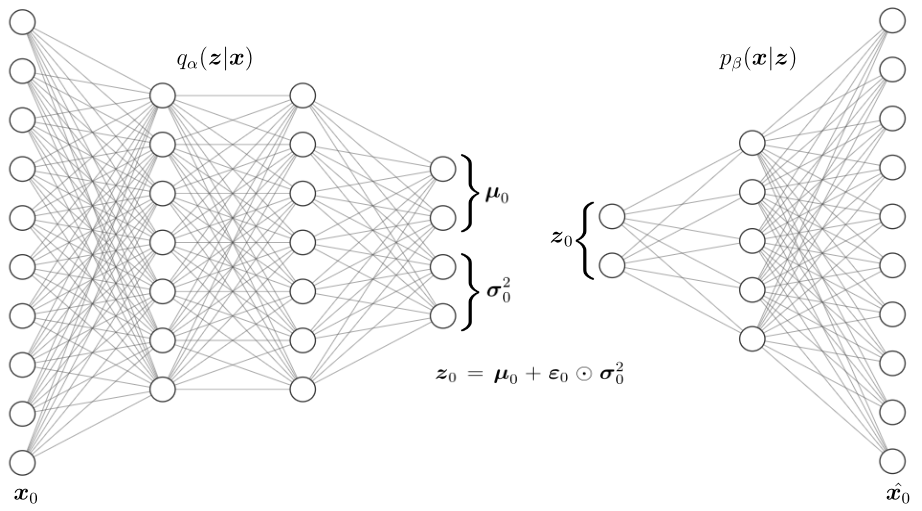
\includegraphics[width=.95\textwidth]{img/vae_visual.png}
  \caption{Visualization of a VAE architecture with $n=10$ and $d=2$.}
  \label{fig:vae_visual}
\end{figure}
The VAE architecture is summarized in Figure \ref{fig:vae_visual}. Note that the VAE does not need to be symmetric; the encoder and decoder can have a different number of hidden layers of different sizes.



